\chapter{Packing the Treasure Trunk: Data Structures}

\begin{figure}[h!]
    \centering
    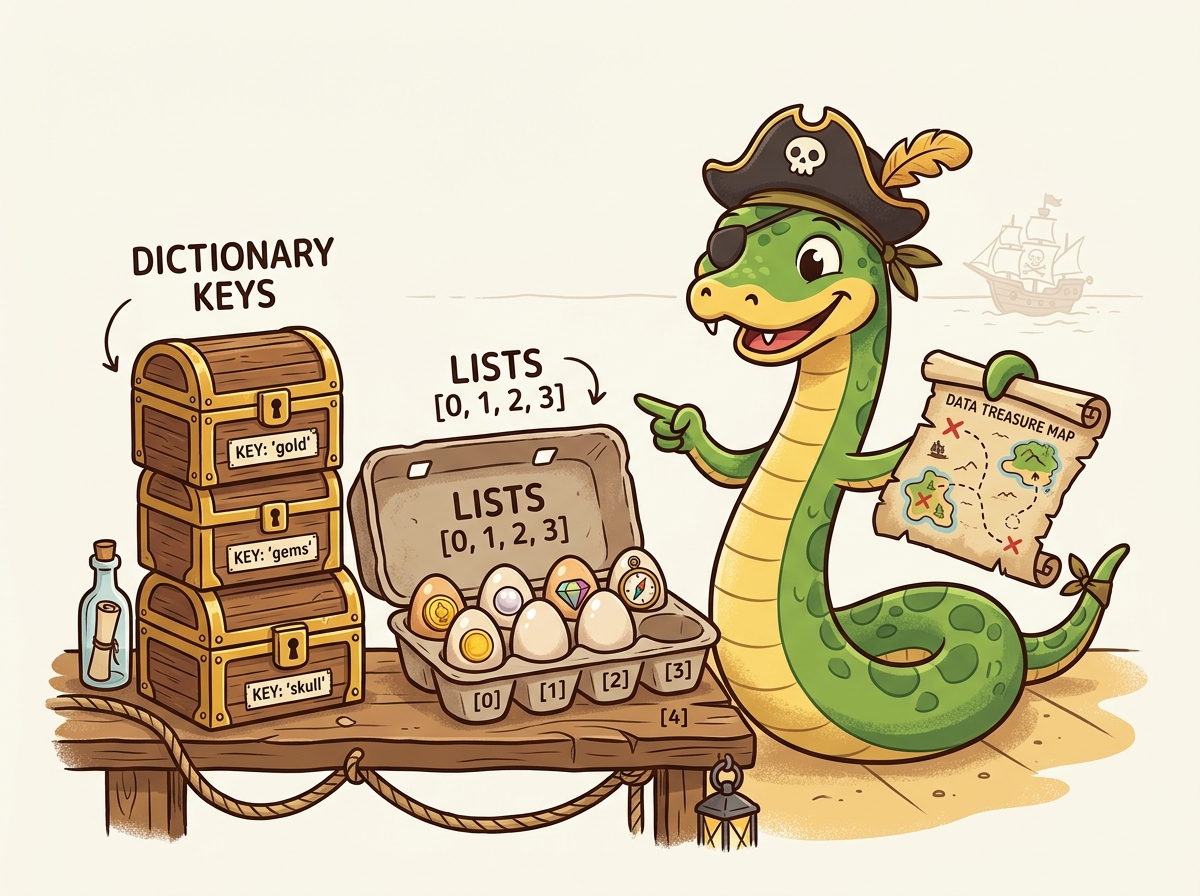
\includegraphics[width=0.75\textwidth]{images/ch5_treasure_chest.jpg}
    \caption{Python data structures organize your data like egg cartons (Lists) and treasure chests (Dictionaries).}
\end{figure}

\section{Beyond Single Variables}

Storing single numbers in individual Tupperware containers is fine for beginners. But what if you have a list of $10,000$ high scores or a map of user profile settings? You need Python's built-in \textbf{data structures}!

\section{Lists: The Infinite Shopping Cart}

A \textbf{list} is an ordered, mutable sequence of items enclosed in square brackets \texttt{[]}.

\begin{pycode}{List Basics}
inventory = ["Magic Wand", "Health Potion", "Shield", "Dragon Tooth"]

# Accessing items (Zero-indexed!)
print("First item:", inventory[0])    # Magic Wand
print("Last item:", inventory[-1])    # Dragon Tooth

# Modifying items
inventory.append("Spellbook")         # Add to end
inventory.remove("Shield")            # Remove by value
print("Updated Inventory:", inventory)
\end{pycode}

\section{Tuples: Carved in Stone}

A \textbf{tuple} is like a list, but it is \textbf{immutable} (unchangeable). Enclosed in round parentheses \texttt{()}.

\begin{pycode}{Tuple Demo}
screen_resolution = (1920, 1080)
# Trying screen_resolution[0] = 3840 will crash with TypeError!
print(f"Width: {screen_resolution[0]}, Height: {screen_resolution[1]}")
\end{pycode}

\section{Dictionaries: Secret Key-Value Maps}

A \textbf{dictionary} stores data in \textbf{key: value} pairs, enclosed in curly braces \texttt{\{\}}. Instead of numeric positions like \texttt{[0]}, you access values by their unique key!

\begin{pycode}{Dictionary Basics}
hero_stats = {
    "name": "Sir Python",
    "level": 42,
    "hp": 250,
    "class": "Snake Wizard"
}

# Accessing and modifying dictionary values
print("Hero Level:", hero_stats["level"])
hero_stats["hp"] += 50   # Drink health potion!
hero_stats["mana"] = 180  # Add new key-value pair

print("Updated Stats:", hero_stats)
\end{pycode}

\section{Sets: Duplicate-Destroying Bouncers}

A \textbf{set} is an unordered collection of unique elements. If you try to add duplicates, a set silently throws them into the trash!

\begin{pycode}{Set Magic}
raw_tags = ["python", "code", "python", "snake", "code", "magic"]
unique_tags = set(raw_tags)
print("Unique Tags:", unique_tags)
\end{pycode}

\section{Code Example: Word Frequency Counter}

Here is how dictionaries and loops collaborate to count how frequently words appear in a sentence.

\begin{pycode}{Word Frequency Counter}
sentence = "python is fun and python is powerful and python is fast"
words = sentence.split()
counts = {}

for word in words:
    if word in counts:
        counts[word] += 1
    else:
        counts[word] = 1

for word, freq in counts.items():
    print(f" - '{word}': {freq} time(s)")
\end{pycode}

\begin{snakesnack}{List Comprehensions: Pythonic Elegance}
Transforming one list into another in a single sleek line of code:
\begin{lstlisting}[language=Python]
numbers = [1, 2, 3, 4, 5]
squares = [x**2 for x in numbers if x % 2 == 0]
print(squares) # Output: [4, 16]
\end{lstlisting}
\end{snakesnack}

\section{Practice Problems \& Exercises}

Unpack your data structures with these 3 practice challenges!

\begin{snakelab}{Problem 5.1: High Score Leaderboard (Easy)}
Given a list of test scores \texttt{scores = [88, 95, 72, 100, 85, 91]}, write code to:
\begin{itemize}
    \item Sort the list in descending order.
    \item Extract the top 3 highest scores using list slicing (\texttt{[:3]}).
    \item Print the average of those top 3 scores!
\end{itemize}
\end{snakelab}

\begin{pycode}{Solution 5.1: High Score Leaderboard}
scores = [88, 95, 72, 100, 85, 91]

scores.sort(reverse=True)
top_3 = scores[:3]
average_top_3 = sum(top_3) / len(top_3)

print("Sorted Leaderboard:", scores)
print("Top 3 Scores:", top_3)
print(f"Top 3 Average: {average_top_3:.1f}")
\end{pycode}

\begin{snakelab}{Problem 5.2: Recipe Ingredient Matcher (Medium)}
Given two sets of ingredients:
\texttt{recipe\_a = \{"flour", "sugar", "eggs", "butter", "vanilla"\}}
\texttt{recipe\_b = \{"flour", "cocoa", "eggs", "butter", "milk"\}}
Write set operations to find:
\begin{enumerate}
    \item Common ingredients in both recipes (intersection \texttt{\&}).
    \item All unique ingredients required across both recipes (union \texttt{\textbar}).
\end{enumerate}
\end{snakelab}

\begin{pycode}{Solution 5.2: Recipe Ingredient Matcher}
recipe_a = {"flour", "sugar", "eggs", "butter", "vanilla"}
recipe_b = {"flour", "cocoa", "eggs", "butter", "milk"}

common = recipe_a & recipe_b
all_unique = recipe_a | recipe_b

print("Common Ingredients:", common)
print("All Required Ingredients:", all_unique)
\end{pycode}

\begin{snakelab}{Problem 5.3: Student Grade Dictionary Lookup (Spicy)}
Create a dictionary mapping student names to lists of grades:
\texttt{grades = \{"Alice": [90, 85, 92], "Bob": [75, 80, 70], "Charlie": [95, 98, 100]\}}
Iterate through the dictionary and print each student's name and their calculated final grade average!
\end{snakelab}

\begin{pycode}{Solution 5.3: Student Grade Lookup}
grades = {
    "Alice": [90, 85, 92],
    "Bob": [75, 80, 70],
    "Charlie": [95, 98, 100]
}

print("--- STUDENT FINAL GRADES ---")
for student, mark_list in grades.items():
    avg = sum(mark_list) / len(mark_list)
    print(f"Student: {student:8s} | Average: {avg:.1f}%")
\end{pycode}
